\documentclass[11pt,a4paper]{article}
\usepackage[margin=25mm]{geometry}
\usepackage{amsmath,amssymb}
\usepackage{xcolor}
\usepackage{array}
\definecolor{outA}{HTML}{145487}
\definecolor{outB}{HTML}{8A4517}
\definecolor{outC}{HTML}{096556}
\newcommand{\ca}[1]{\textcolor{outA}{#1}}
\newcommand{\cb}[1]{\textcolor{outB}{#1}}
\newcommand{\ccol}[1]{\textcolor{outC}{#1}}
\newcommand{\abc}[3]{\ca{#1},\,\cb{#2},\,\ccol{#3}}
\newenvironment{weights}{\left[\begin{array}{>{\color{outA}}r>{\color{outB}}r>{\color{outC}}r}}{\end{array}\right]}
\usepackage[T1]{fontenc}
\usepackage{lmodern,microtype,booktabs,tikz,listings,titlesec,fancyhdr,needspace}
\definecolor{ink}{HTML}{19364B}
\definecolor{muted}{HTML}{4E6271}
\definecolor{panel}{HTML}{EFF4F6}
\definecolor{rulegray}{HTML}{CCD8DD}
\usepackage[bookmarksnumbered,colorlinks,linkcolor=ink,urlcolor=outA,citecolor=outC]{hyperref}
\hypersetup{pdftitle={CPU kernels for sparse ternary matrix multiplication},
 pdfsubject={RSR, SSR and TCSC algorithms and CPU implementation}}
\setlength{\parindent}{0pt}
\setlength{\parskip}{0.48em}
\setlength{\emergencystretch}{1.3em}
\setcounter{tocdepth}{1}
\raggedbottom
\widowpenalty=8000 \clubpenalty=8000
\titleformat{\section}{\Large\sffamily\bfseries\color{ink}}{\thesection}{0.6em}{}
\titleformat{\subsection}{\large\sffamily\bfseries\color{ink}}{\thesubsection}{0.5em}{}
\titlespacing*{\section}{0pt}{1.3em}{0.45em}
\titlespacing*{\subsection}{0pt}{1em}{0.35em}
\pagestyle{fancy}\fancyhf{}
\fancyhead[L]{\sffamily\small\color{muted}Sparse ternary matrix multiplication}
\fancyhead[R]{\sffamily\small\color{muted}\nouppercase{\leftmark}}
\renewcommand{\sectionmark}[1]{}
\fancyfoot[R]{\sffamily\small\thepage}
\setlength{\headheight}{15pt}
\renewcommand{\headrulewidth}{0.3pt}
\newcommand{\familymark}[1]{\markboth{#1}{}}
\newcommand{\code}[1]{\texttt{\detokenize{#1}}}
\lstset{language=C++,basicstyle=\small\ttfamily,keywordstyle=\color{outA}\bfseries,
 commentstyle=\color{muted}\itshape,showstringspaces=false,keepspaces=true,
 columns=fullflexible,backgroundcolor=\color{panel},frame=l,framerule=1pt,
 rulecolor=\color{outA},xleftmargin=7pt,framexleftmargin=6pt,
 aboveskip=0.6em,belowskip=0.5em,breaklines=true}
\renewcommand{\arraystretch}{1.13}
\newcommand{\diagramcaption}[1]{\par{\small\sffamily\color{muted}#1}\par}
\begin{document}
\thispagestyle{empty}
{\sffamily\large\color{outC}RSR \quad RSR++ \quad SSR \quad TCSC\par}
\vspace{0.6em}
{\sffamily\bfseries\fontsize{28}{32}\selectfont\color{ink} CPU kernels for sparse ternary\\matrix multiplication\par}
\vspace{0.5em}
{\large How groups of weights become sums, memory reads and parallel work\par}
\medskip
Given \(Y=XW\), a weight of \(+1\) copies an activation into a sum, a
\(-1\) subtracts it, and a zero contributes nothing. The hard part is deciding
which activations to fetch and how often to visit the same data. The three
families in this guide answer those questions at different stages:
\begin{description}
\item[RSR / RSR++] Find rows with the same pattern. Compute their sum once,
then reconstruct the output columns.
\item[SSR] Skip input rows that cannot affect a binary block, then compute
several input rows together when the CPU and shape permit it.
\item[TCSC] Start with an output column. Visit only the inputs with positive
or negative weights, then align work across columns.
\end{description}
\vfill
{\large\sffamily\bfseries\color{ink}Reading map\par}
\begin{center}
\begin{tabular}{@{}p{.76\linewidth}r@{}}
\toprule
\hyperref[sec:first]{From a matrix product to binary group sums} & \pageref{sec:first}\\
\hyperref[sec:fold]{RSR and the RSR++ folding tree} & \pageref{sec:fold}\\
\hyperref[sec:binary]{Direct scatter and the RSR-core CPU loops} & \pageref{sec:binary}\\
\hyperref[sec:ternary]{Signed groups and mask-based SIMD} & \pageref{sec:ternary}\\
\hyperref[sec:ssr]{SSR preprocessing and the shortened tree} & \pageref{sec:ssr}\\
\hyperref[sec:ssrcpu]{SSR basic, unrolled and specialized tree kernels} & \pageref{sec:ssrcpu}\\
\hyperref[sec:tcsc]{TCSC lists, paired contributions and grouped gathers} & \pageref{sec:tcsc}\\
\hyperref[sec:timing]{Interpreting single-thread and multicore timings} & \pageref{sec:timing}\\
\bottomrule
\end{tabular}
\end{center}
\vfill
\clearpage
\familymark{RSR and RSR++}
\Needspace{7\baselineskip}
\section{One product, two opportunities for reuse}\label{sec:first}
We compute \(Y=XW\), with FP32 activations \(X\in\mathbb R^{M\times K}\),
weights \(W\in\{-1,0,1\}^{K\times N}\), and outputs \(Y\in\mathbb R^{M\times N}\).
Each row \(\mathbf x\) of \(X\) produces one row \(\mathbf y=\mathbf xW\).
Divide the output columns into blocks of width \(b\). Thus \(K\) counts input
activations and \(b\) counts outputs computed together.

Throughout the examples, \(\ca{A}\) is blue, \(\cb{B}\) is brown, and
\(\ccol{C}\) is green. Read a three-bit pattern in that order:
\(\ca{1}\cb{0}\ccol{1}\) sends its group sum to \(\ca{A}\) and \(\ccol{C}\).
Column positions and labels carry the same information in a monochrome printout.

Start with one binary block. Label its columns \(A,B,C\) from left to right.
\[
\mathbf x=\begin{bmatrix}2&3&5&7&11&13\end{bmatrix},\qquad
W=\begin{weights}
1&0&1\\0&1&1\\1&0&1\\1&1&0\\0&1&1\\1&1&1
\end{weights}.
\]
Reading down each column gives the reference calculation:
\[
\begin{aligned}
\ca{y_A}&=x_1+x_3+x_4+x_6=27,\\
\cb{y_B}&=x_2+x_4+x_5+x_6=34,\\
\ccol{y_C}&=x_1+x_2+x_3+x_5+x_6=34.
\end{aligned}
\]
In symbols, for an output column \(j\) in this block,
\[
  y_j=\sum_{i=1}^K x_i W_{ij}
     =\sum_{\text{patterns }p} p_j
       \underbrace{\sum_{i\in G_p} x_i}_{u_p}.
\]
The first sum walks the column in its original order. The second first
collects the terms with the same coefficient pattern. Expanding the inner
sum gives the same real-number product. The two evaluation orders can round
differently in FP32.

The sum \(x_1+x_3\) appears in both \(A\) and \(C\). We can predict this
from the weights alone: rows 1 and 3 are identical across the block.
Likewise \(x_2+x_5\) appears in both \(B\) and \(C\).

For a pattern \(p\), let \(G_p\) be the set of rows with pattern \(p\) within
the block, and let \(u_p=\sum_{i\in G_p}x_i\). Preparing the weights determines
the groups once. Each new input requires fresh values of \(u_p\).
\[
\begin{array}{c|c|c|c}
p&G_p&u_p&\text{output destinations}\\\hline
011&\{2,5\}&3+11=14&B,C\\
101&\{1,3\}&2+5=7&A,C\\
110&\{4\}&7&A,B\\
111&\{6\}&13&A,B,C
\end{array}
\]
One possible permutation is \((2,5\mid1,3\mid4\mid6)\).
The bars mark segment boundaries. Reading the indices between two bars
visits all members of one group. The input vector stays in its original
order. The paper calls this a \emph{segmented sum} \cite{paper}.

\Needspace{7\baselineskip}
\section{RSR and RSR++ on the same block}\label{sec:fold}
\Needspace{5\baselineskip}
\subsection{RSR reconstructs the output from the pattern matrix}
Order the binary patterns from \(000\) through \(111\), assigning zero to
empty groups. The group sums form the row vector
\(\mathbf u=[0,0,0,14,0,7,7,13]\). With one row per possible pattern,
RSR computes
\[
\mathbf y=\mathbf uP_b,\qquad
P_3=\begin{weights}
0&0&0\\0&0&1\\0&1&0\\0&1&1\\
1&0&0\\1&0&1\\1&1&0\\1&1&1
\end{weights}.
\]
Here \(P_b\) has shape \(2^b\times b\). Its rows encode all possible
patterns; \(\mathbf u\) supplies the data-dependent coefficients.
For instance \(u_{011}=14\) contributes \(14[0,1,1]\), namely
\([\abc{0}{14}{14}]\), to the product. The identical pattern will have
different group sums when a new activation row arrives.

The first column selects \(u_{100}+u_{101}+u_{110}+u_{111}=27\).
The second selects \(u_{010}+u_{011}+u_{110}+u_{111}=34\).
Both expressions contain \(u_{110}+u_{111}\). RSR has reused sums of
\emph{activations}; RSR++ also reuses sums of \emph{groups}.

\Needspace{5\baselineskip}
\subsection{RSR++ computes one output and discards one bit per level}
First compute \(C\). Its bit is 1 in the second member of each adjacent pair:
\[
\ccol{y_C}=u_{001}+u_{011}+u_{101}+u_{111}=0+14+7+13=34.
\]
Once \(C\) is complete, \(110\) and \(111\) have identical effects on the
remaining outputs: both contribute to \(A\) and \(B\). Merge each adjacent
pair and label the result by its two surviving bits:
\[
\begin{aligned}
t_{00}&=u_{000}+u_{001}=0,& t_{01}&=u_{010}+u_{011}=14,\\
t_{10}&=u_{100}+u_{101}=7,& t_{11}&=u_{110}+u_{111}=20.
\end{aligned}
\]
Now the last surviving bit denotes \(B\). Select the entries ending in 1,
then merge pairs again:
\[
\cb{y_B}=t_{01}+t_{11}=34,\qquad
q_0=t_{00}+t_{01}=14,\qquad q_1=t_{10}+t_{11}=27.
\]
The sole surviving bit denotes \(A\), so \(\ca{y_A}=q_1=27\).
The following dependency diagram traces only the contributions to \(A\)
and \(B\) after \(C\) has been computed.
\begin{center}
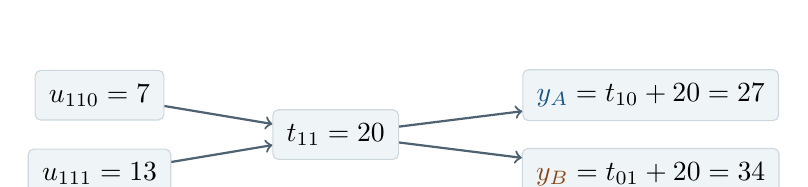
\begin{tikzpicture}[x=1cm,y=1cm,box/.style={draw=rulegray,fill=panel,rounded corners=2pt,inner sep=5pt},arr/.style={->,draw=muted,thick}]
\node[box] (a) at (0,0) {\(u_{110}=7\)};
\node[box] (b) at (0,-1) {\(u_{111}=13\)};
\node[box] (t) at (3,-.5) {\(t_{11}=20\)};
\node[box] (ya) at (7,0) {\(\ca{y_A}=t_{10}+20=27\)};
\node[box] (yb) at (7,-1) {\(\cb{y_B}=t_{01}+20=34\)};
\draw[arr] (a)--(t);\draw[arr] (b)--(t);\draw[arr] (t)--(ya);\draw[arr] (t)--(yb);
\end{tikzpicture}
\end{center}
The intermediate 20 contributed to both \(B\) and \(A\).
At width \(b\), the lengths processed are \(2^b,2^{b-1},\ldots,2\).
Their geometric sum gives \(O(2^b)\) reconstruction work per block, compared
with \(O(b2^b)\) for the explicit pattern product. Both still pay for forming
the group sums, including reading \(K\) activations per binary block and plane.

\paragraph{What the repository runs.}
The local \code{rsr_pp_inference} calls \code{step_three} on each block.
Each level sums odd-indexed entries and makes a second pass to merge pairs.
The block vector is passed by value. A possible optimization would read a
pair once, add its odd member to the current output and write the pair sum
to the next level. The caller could let the routine consume its block
buffer to avoid the copy. These are possible changes to the local baseline.
The three imported RSR-core kernels implement direct output updates.
The upstream CPU catalog describes fused aggregation and scatter variants;
it lists no dedicated CPU implementation of the paper's RSR++ folding tree
\cite{core,guide}. Timings of the RSR++ entry apply to the local implementation.

\Needspace{7\baselineskip}
\section{Binary split v4.2}\label{sec:binary}
\Needspace{5\baselineskip}
\subsection{Finish a group and immediately update its destinations}
For each observed binary pattern, preprocessing saves the positions of its
ones. Once a group sum is ready, v4.2 adds it to those positions and moves
on. This operation is a \emph{scatter-add}. Follow the complete execution:
\[
\begin{array}{c|r|l|c}
p&u_p&\text{destinations}&(\ca{y_A},\cb{y_B},\ccol{y_C})\text{ after updates}\\\hline
 & &\text{initialize}&(0,0,0)\\
011&14&\cb B,\ccol C&(\abc{0}{14}{14})\\
101&7&\ca A,\ccol C&(\abc{7}{14}{21})\\
110&7&\ca A,\cb B&(\abc{14}{21}{21})\\
111&13&\abc{A}{B}{C}&(\abc{27}{34}{34})
\end{array}
\]
Forming \(14=x_2+x_5\) reads two activations. Distributing that 14 takes
two output updates. If one hundred rows shared \(011\), forming the sum
would read one hundred activations, but distributing the result would still
take exactly two updates.

In C++-style pseudocode, one fused iteration has this data flow:
\Needspace{9\baselineskip}
\begin{lstlisting}
float group_sum = 0;
for (int i = begin; i < group_end[g]; ++i)
    group_sum += x[perm[i]];
for (int j = offsets[g]; j < offsets[g + 1]; ++j)
    out[dest[j]] += group_sum;
begin = group_end[g];
\end{lstlisting}
The first loop length counts rows with this pattern. The second counts
active output positions. Neither bound can be inferred from the other.
For example, a hundred rows of pattern 001 produce one destination, whereas
a single row of pattern 111 produces three. This is why the column-block
pattern distribution matters in addition to the overall weight sparsity.

For one plane and block, let \(\mathcal P\) contain the observed patterns.
The number of scalar scatter-adds is
\[
D=\sum_{p\in\mathcal P}\operatorname{popcount}(p),
\]
where popcount counts the ones. Here \(D=2+2+2+3=9\). An all-\(011\) block
needs just two updates. If every pattern occurs, each of the \(b\) positions
is 1 in \(2^{b-1}\) patterns, giving \(D=b2^{b-1}\), or 12 at \(b=3\).
This counts output updates only. There are also input reads, group boundaries
and loop overhead. The code sums an observed all-zero group even though its
destination list is empty. A small \(D\) explains an opportunity for savings;
it cannot predict elapsed time alone.

\Needspace{5\baselineskip}
\subsection{Two binary planes for ternary weights}
Change the first row of our original binary matrix to \((1,-1,1)\).
Let the resulting matrix be \(W_{\rm tern}\).
Set \(W^+_{ij}=\mathbf{1}_{(W_{{\rm tern},ij}=1)}\) and
\(W^-_{ij}=\mathbf{1}_{(W_{{\rm tern},ij}=-1)}\). The first row decomposes as
\[
[1,-1,1]=[1,0,1]-[0,1,0].
\]
The entire positive plane is our original matrix. The negative plane contains
a single 1 at row 1, column \(B\). With \(x_1=2\), the wrapper computes
\[
\mathbf xW_{\rm tern}
=\mathbf xW^+-\mathbf xW^-
=[27,34,34]-[0,2,0]=[27,32,34].
\]
Both portable baselines also use this two-plane identity. Each plane has
its own groups and permutation. Each block therefore visits the input once
on each plane, and the wrapper subtracts the two output vectors.

\Needspace{7\baselineskip}
\section{How RSR-core executes a group sum}
The shortened C++ examples below explain the hot loop. Array offsets are
zero-based; the numbered matrix rows above are one-based.
\Needspace{5\baselineskip}
\subsection{Contiguous metadata and indirect input reads}
Suppose two groups have input indices \((8,2,15)\) and \((4,9)\),
and destinations \((B,C)\) and \((A,C)\). Encode \(A,B,C\) as \(0,1,2\).
\Needspace{7\baselineskip}
\begin{lstlisting}
perm            = [8, 2, 15, 4, 9]
group_ends      = [3, 5]
scatter_rows    = [1, 2, 0, 2]
scatter_offsets = [0, 2, 4]
\end{lstlisting}
For group zero, read permutation positions \(0,1,2\), then update destinations
at scatter positions \(0,1\). The next group continues where the first ended.
The metadata arrays are contiguous. A cache line containing one entry also
brings nearby entries that will be needed soon. Each local destination uses
one byte. The activation reads \(x[8],x[2],x[15]\) can still be far apart.
For example, group zero computes \(x[8]+x[2]+x[15]\) once and adds it
to \(B,C\). Group one computes \(x[4]+x[9]\) and adds it to \(A,C\).
If the sums are 10 and 7, an initially zero output becomes
\([\abc{7}{10}{17}]\). The exclusive ends 3 and 5 count entries consumed
in \code{perm}. The offsets 0, 2 and 4 mark boundaries in the separate
list of destinations.

The block width \(b\) counts columns of \(W\) examined together.
The group length \code{len = end - start} counts rows of \(W\) with a
particular pattern on those columns. A two-column block can have 100 rows
with pattern \((1,0)\), giving \(b=2\) and \(\mathrm{len}=100\).
Adding a column can split that group if its rows differ on the new column.

The local builder counts occurrences of each binary or ternary code, uses
prefix counts to place row indices, and retains group descriptors only for
observed codes. The temporary counting table still has \(2^b\) or \(3^b\)
entries. The portable baseline sorts indices by pattern.

\Needspace{5\baselineskip}
\subsection{Short groups and independent accumulators}
A register is a small storage location inside a core. An accumulator is a
variable holding a running total, which the compiler can keep in a register.
In a simple loop the next accumulator value needs the previous one:
\Needspace{6\baselineskip}
\begin{lstlisting}
float sum = 0.0f;
for (int i = begin; i < end; ++i)
    sum += x[perm[i]];
\end{lstlisting}
The contiguous read of \code{perm[i]} discovers where to read \code{x}.
The processor can start independent reads early, but each update of
\code{sum} needs the preceding result. This explains why the imported
kernel has separate strategies for short and long groups.

Suppose the three activation values are 4, 7 and 2. The running total
goes from 0 to 4, then 11, then 13. The core can begin fetching the 7
while the first addition is in flight. Adding that 7 to the running total
requires the result 4.

For lengths 1--4 the kernel branches to the corresponding case:
\Needspace{9\baselineskip}
\begin{lstlisting}
switch (len) {
case 4: sum += x[perm[start + 3]]; [[fallthrough]];
case 3: sum += x[perm[start + 2]]; [[fallthrough]];
case 2: sum += x[perm[start + 1]]; [[fallthrough]];
case 1: sum += x[perm[start]];     break;
}
\end{lstlisting}
A group of length three enters at case 3 and executes three loads and
additions. There is no counter test between additions. The branch hint
\code{__builtin_expect(len <= 4, 1)} tells the compiler that short groups
are expected to be common. Their actual frequency depends on the matrix.

For the first group above, fallthrough visits cases 3, 2 and 1 and
reads \(x[15],x[2],x[8]\) in that order. Four is an implementation
choice: extending the switch to length 100 would require 100 cases.
In the branch hint, 1 means the comparison is expected to be true.
The actual length still selects the branch each time.

For longer groups, write \(a_j=x[\mathrm{perm}[i+j]]\) for the values at
the current permutation position \(i\). One full iteration does this:
\Needspace{5\baselineskip}
\begin{lstlisting}
s0 += a0 + a1;    s1 += a2 + a3;
s2 += a4 + a5;    s3 += a6 + a7;
\end{lstlisting}
At \(i=0\), \(a_0=x[\mathrm{perm}[0]]\) and
\(a_1=x[\mathrm{perm}[1]]\). If the eight values are \(1,\ldots,8\),
the four initially zero totals become \(3,7,11,15\). On the next
iteration \(a_0\) denotes the ninth value and each accumulator retains
its previous total.

The loop advances \(i\) by eight. A group of 18 uses two such iterations
and a two-element tail. A group of length 5--7 uses only the tail loop.
Unrolling reduces loop-control work. The four accumulators shorten the
dependency chain: a core can issue work for \code{s1} before the latest
update to \code{s0} finishes. A single thread is sufficient. The four
sums are combined as \((s_0+s_1)+(s_2+s_3)\) before any tail additions.
Regrouping FP32 additions can change rounding.

\Needspace{5\baselineskip}
\subsection{Prefetch and parallel blocks}
A cache holds small chunks of recently accessed memory close to the CPU.
Successive indices in \code{perm} share such chunks. The activations they
point to may be scattered far enough apart to occupy different chunks.

To evaluate \code{x[perm[i]]}, the core first needs the index and then the
activation at that index. In AVX2 builds, v4.2 issues prefetch hints for
\code{x[perm[i+64]]} and the corresponding positions \(i+66,i+68,i+70\)
when sufficiently far from the group end. If \(\mathrm{perm}[i+64]=900\),
the requested cache line contains \(x[900]\). The distance of 64 is measured
in permutation entries. Useful work on the current group can overlap the
wait for a future load. Small groups never enter this path, and an already
cached input may gain little. The v4.2 scatter itself is scalar.

Here is the long-group loop in an AVX2 build of v4.2. The four partial
sums start at zero. With \(i=0\), the hints prepare values for the
iteration eight trips ahead while the additions consume positions 0--7.
\begin{lstlisting}
int i = start;
for (; i + 7 < end; i += 8) {
    if (i + 64 + 7 < end) {
        _mm_prefetch((const char*)&x[perm[i+64]], _MM_HINT_T0);
        _mm_prefetch((const char*)&x[perm[i+66]], _MM_HINT_T0);
        _mm_prefetch((const char*)&x[perm[i+68]], _MM_HINT_T0);
        _mm_prefetch((const char*)&x[perm[i+70]], _MM_HINT_T0);
    }
    s0 += x[perm[i  ]] + x[perm[i+1]];
    s1 += x[perm[i+2]] + x[perm[i+3]];
    s2 += x[perm[i+4]] + x[perm[i+5]];
    s3 += x[perm[i+6]] + x[perm[i+7]];
}
float sum = (s0 + s1) + (s2 + s3);
for (; i < end; ++i) sum += x[perm[i]];
\end{lstlisting}
At length 5 the group enters the long branch. At length 8 the first
eight-value iteration runs. The first prefetch requires 72 remaining
entries because \(i+71<\mathrm{end}\). At exactly 72 only the first
iteration issues the four hints. The second has 64 entries left.

With OpenMP enabled, static scheduling assigns disjoint output blocks to
threads. Each thread owns the outputs of its block, so scatter needs no
atomic updates. The local wrapper traverses the \(M\) activation rows
sequentially. Thus the matrix product consists of repeated matrix--vector
kernel calls with shared prepared weights. For example, one thread can own
columns \(A,B\) and another \(C,D\). Every update to \(B\) then comes
from its owner. Moving to the next row of \(X\) changes the activation
values and reuses the same permutation and destinations.

\Needspace{7\baselineskip}
\section{Direct ternary groups: v3.1 and v3.3}\label{sec:ternary}
\Needspace{5\baselineskip}
\subsection{v3.1 attaches a sign to each destination}
To see why direct ternary grouping can change the groups themselves, use
\[
\mathbf x=\begin{bmatrix}2&3&5&7\end{bmatrix},\qquad
W=\begin{weights}1&0&-1\\1&-1&0\\1&0&-1\\0&1&-1\end{weights}.
\]
Rows 1 and 3 have the same complete pattern. Their sum \(s=2+5=7\)
contributes \(+7\) to \(A\) and \(-7\) to \(C\). Each destination has a sign:
\Needspace{5\baselineskip}
\begin{lstlisting}
for (int j = offsets[g]; j < offsets[g + 1]; ++j)
    out[columns[j]] += signs[j] * sum;
\end{lstlisting}
Following the groups in the order below gives the full product:
\[
\begin{array}{c|c|c|c}
p&G_p&\text{signed contribution}&\text{running output}\\\hline
(1,0,-1)&\{1,3\}&(7,0,-7)&(7,0,-7)\\
(1,-1,0)&\{2\}&(3,-3,0)&(10,-3,-7)\\
(0,1,-1)&\{4\}&(0,7,-7)&(10,4,-14)
\end{array}
\]
Check by columns: \(\ca{y_A}=2+3+5=10\), \(\cb{y_B}=-3+7=4\),
\(\ccol{y_C}=-2-5-7=-14\). Group order above is for exposition.

On the positive plane, v4.2 would merge rows 1, 2 and 3 into one \(100\)
group, contributing 10 to \(A\) in one update. Direct ternary grouping
separates row 2 because its negative weight is in \(B\); \(A\) receives
two updates. In return, v3.1 handles the negative contributions in the same
pass. Width six admits 64 binary patterns per plane but 729 signed patterns.
Saving a pass need not halve the runtime.

The builder encodes weights \(0,+1,-1\) as base-three digits \(0,1,2\).
Column \(A\) has place value 1, \(B\) has 3 and \(C\) has 9. Thus
\((+1,0,-1)\) gets code \(1+0\cdot3+2\cdot9=19\). Both matching rows
receive code 19. Their group length is 2 and their activation sum is 7. Permutations and group
ends use 16-bit unsigned indices, halving their bytes per entry relative to
v4.2 and requiring \(K\leq65535\). v3.1 stores a one-byte destination and a
one-byte sign for each active position. Its CPU loop uses the same short-group
switch and four accumulators; the AVX2 prefetch distance is 48 entries.
The first prefetch therefore requires \(48+8=56\) remaining entries.
The explicit signed scatter visits \((A,+1)\) and \((C,-1)\) for the
first group, adding 7 to \(A\) and subtracting 7 from \(C\).

For \(K=5\) rows, a permutation \([1,4,0,2,3]\) and ends \([2,5]\)
would describe groups of two and three rows. The largest row index is 4,
while the last exclusive end is 5. An unsigned 16-bit entry occupies
two bytes and can hold values from 0 through 65535. At \(K=65536\) the
largest row index still fits but the last end overflows. This is why
the limit on \(K\) applies even with zero-based row indices.

\Needspace{5\baselineskip}
\subsection{v3.3 represents the same destinations by two masks}
Keep the same matrix. For the first group \(p=(1,0,-1)\), the positive mask
selects \(A\) and the negative mask selects \(C\). With bit zero assigned
to \(A\), the integer mask values are 1 and 4, respectively.
The scalar path repeatedly locates the least significant set bit, updates
that output and clears the bit. Each group stores two 16-bit masks.
A group with many active columns needs the same four mask bytes as a group
with one active column. Sparse lists can still be compact for short lists.

Bits for \(A,B,C\) have values \(1,2,4\). The negative mask 4 therefore
tells the kernel \emph{where} to subtract. The group sum 7 supplies the
amount. With \(d\) active columns the v3.1 lists use \(2d\) bytes for
destinations and signs. The v3.3 masks use four bytes per group: for
one active column the comparison is two versus four bytes, and for three
it is six versus four.

For a positive mask of decimal 5, the set bits are \(0\) and \(2\).
The scalar walk visits exactly two destinations. The bit operation in
the last line below removes the lowest set bit: binary \(101\) becomes
\(100\), then \(000\).
\Needspace{9\baselineskip}
\begin{lstlisting}
// One positive mask; the negative-mask loop subtracts instead.
while (mask != 0) {
    unsigned lane = __builtin_ctz(unsigned(mask));
    out[lane] += group_sum;
    mask &= mask - 1;
}
\end{lstlisting}
The nonzero test ensures that counting trailing zero bits always yields
a destination. For a given pattern, this path only touches active columns.

For example, binary \(100\) has two trailing zeros, so the scalar walk
updates lane 2 (\(C\)). Binary \(000\) has no destination and terminates
the walk.

The SIMD path expands the low eight bits of a mask through a 256-entry table.
Each entry contains eight FP32 lane coefficients. For our group the two
expanded vectors begin \([1,0,0]\) and \([0,0,1]\); subtracting gives
\([1,0,-1]\). Broadcasting the scalar group sum 7 produces the update
\[
\mathbf y_{\rm block}\gets \mathbf y_{\rm block}+7[\abc{1}{0}{-1}].
\]
Expansion turns each bit into its own FP32 value, 0.0 or 1.0.
Eight bits admit \(2^8=256\) combinations, hence one table row per mask.
In binary \(100\), bit zero is printed on the right. The expanded
coefficients for \(A,B,C\) are listed in column order as \([0,0,1]\).
Broadcasting copies 7 into every lane. For running totals \([10,20,30]\),
the update gives \([10+7,20+0,30-7]=[17,20,23]\).

The kernel accumulates across groups in vector registers and stores the
active output lanes at the end. SIMD acts across \emph{columns};
the indirect input reads still form a separate aggregation step. AVX2 uses
one eight-lane register, with fused multiply-add when enabled. NEON uses
two four-lane registers. The local wrapper accepts widths 1--8; the vector
path depends on build flags and width (AVX2 at widths 1--8, NEON at 5--8).
AVX2 is an x86 SIMD instruction-set extension. Arm NEON performs the
eight FP32 operations using two 128-bit vectors. At width eight, a
19-column matrix has blocks containing 8, 8 and 3 real output columns.
The build and width determine the path independently of group mask density.
Other supported cases use the scalar mask walk. The vector path loads two
coefficient rows, subtracts them lane by lane and broadcasts the same group
sum to all lanes. It trades a fixed amount of vector work for the variable
number of indexed updates in the scalar loop. A short sparse mask and a
dense mask can therefore favor different paths on the same processor.
For one active column the scalar walk performs one update, and for eight
it performs eight. The vector arithmetic covers the same lanes in either
case. Which path is faster on a given matrix is a measurement question.

\Needspace{7\baselineskip}
\section{Interpreting the RSR comparisons}
All five entries compute the same \(Y=XW\) on the same saved FP32 inputs and
ternary weights. The harness validates the output against FP64 accumulation
before timing. If \(b\) does not divide \(N\), the wrappers retain the first
\(N\) output columns after processing the final padded block. This permits
comparisons on rectangular as well as square weights \cite{local}.

\begin{itemize}
\item \textbf{RSR versus RSR++.} Holding the binary planes and group sums
fixed exposes the change from explicit pattern multiplication to folding.
Differences in temporary allocation and copying also affect the measured call.
\item \textbf{RSR versus v4.2.} Both use the same binary decomposition.
This tests the combined effect of visiting observed groups, fusing aggregation
with sparse scatter, and engineering the CPU loops.
\item \textbf{v4.2 versus v3.1.} Both update destination lists directly.
The comparison exposes the trade between two binary passes and potentially
more distinct signed groups, alongside the change in index size.
\item \textbf{v3.1 versus v3.3.} Both form exactly the same ternary groups.
The main change is how the sum reaches the outputs: signed lists versus
masks with scalar bit iteration or SIMD. The reported backend and block
width matter when interpreting this pair.
\end{itemize}

The sweep varies sparsity at fixed shape and size at fixed sparsity. Two
matrices with the same zero fraction can place their nonzeros in different
columns and generate different patterns. The recorded distinct nonzero
pattern count helps interpret the timings; it does not directly measure
the per-block scatter-add count \(D\).

Preprocessing time and stored weight/metadata bytes are reported separately.
Warm calls reuse prepared weights. The timed scope includes the public
multiply call, its internal temporaries and required output copies. This
models repeated inference with fixed weights. For a one-off product, setup
cost also matters. For a large activation batch, the row-by-row GEMV wrapper
has different opportunities for reuse from a dedicated multi-row GEMM kernel.
Thread settings and scalar/SIMD backend labels belong alongside the median
call time. None of the work counts above is a measured speedup.

\Needspace{5\baselineskip}
\subsection{Why these three RSR-core kernels belong in the comparison}
RSR-core documents additional CPU choices beyond the three kernels registered
here \cite{guide}. Its earlier binary C kernel uses AVX2 gather on long groups.
Binary v2.4 gathers the permuted input into a contiguous, 64-byte-aligned
buffer per thread; summation can then stream through it, at the cost of
writing and rereading the buffer. Binary v4.2 sums directly through
the permutation. Upstream also provides rectangular and padding adapters.
Ternary v1.4 encodes separate positive and negative bit fields in one group
code and stores signed destination lists. These examples illustrate how
input layout, index traffic and scatter representation can change independently.
These alternatives suggest specific benchmark questions. Holding binary splitting
fixed, v4.2 gives a direct-gather baseline for comparison with the portable RSR
and RSR++. Adding v2.4 would primarily test whether staging permuted activations
in a buffer pays for its extra memory traffic. That is a useful narrower
experiment. The rectangular wrapper reuses the binary inference kernel, so a
second timing label for it would duplicate the computation on the same shape.

Adding v3.1 answers a different question: what happens if we group directly by
the entire ternary pattern and read each activation once per block? Its signed lists also give a
baseline for v3.3 on exactly the same groups. Comparing only v4.2 and v3.3
would change grouping, index size, destinations and SIMD together. The v3.1
entry makes that comparison easier to interpret. Earlier v1.4 also performs
signed scatter; comparing it with v3.1 would study encoding and metadata in
more detail. The CUDA versions target a different processor and execution
model. These are technical reasons for this selection in an FP32 CPU study;
the relative speeds of omitted kernels would require separate measurements.

\Needspace{11\baselineskip}
\familymark{Sparse Segment Reduction}
\Needspace{7\baselineskip}
\section{SSR: removing work from the zero group}\label{sec:ssr}
SSR keeps the two binary planes and the segmented sums of RSR++ \cite{ssrpaper}.
To see what changes, keep the input vector from Section~\ref{sec:first} but give three
rows of one binary block the pattern \(000\). Let \(L=b=3\), the block width
in the SSR notation. The columns are \(\abc{A}{B}{C}\), in that order.
\[
\mathbf x=\begin{bmatrix}2&3&5&7&11&13\end{bmatrix},\qquad
W_{\rm block}=\begin{weights}
0&0&0\\1&0&1\\0&0&0\\0&1&1\\1&0&1\\0&0&0
\end{weights}.
\]
Reading down each column gives the reference answer:
\[
\ca{y_A}=x_2+x_5=14,\qquad \cb{y_B}=x_4=7,\qquad
\ccol{y_C}=x_2+x_4+x_5=21.
\]
None of the equations uses \(x_1,x_3,x_6\). We can predict this before any
activations arrive because the corresponding weights are all zero.

\Needspace{5\baselineskip}
\subsection{One zero pattern can account for many input reads}
One possible sorted permutation and its reduced form are
\[
\sigma=(\underbrace{1,3,6}_{000}\mid
         \underbrace{4}_{011}\mid\underbrace{2,5}_{101}),\qquad
\sigma'=(\underbrace{4}_{011}\mid\underbrace{2,5}_{101}).
\]
The portable RSR++ computes \(u_{000}=x_1+x_3+x_6=20\).
Dropping this group eliminates three index visits and three activation reads
per input, plane and block. A thousand occurrences of \(000\) would save a
thousand visits. Both occurrences of \(101\) must remain: each supplies
an activation to a useful sum.

The decision is local to a \emph{block and a plane}. A ternary row
\([0,-1,0]=[0,0,0]-[0,1,0]\) can be skipped on the positive plane.
On the negative plane we need its index to subtract the activation from
\(\cb B\). A different block makes its own decision about the same row.

\paragraph{Paper representation and actual storage.}
Algorithm 1 describes saving the reduced permutation \(\sigma'\).
In the project, \code{handle_block_ssr} sorts and retains all \(K\) indices.
Each plane allocates \(K\) permutation entries and \(2^L\) segment boundaries
per block. Inference skips the zero prefix by starting at the first boundary.
For our matrix the actual layout can be illustrated as follows:
\[
\begin{array}{r|rrrrrr}
\text{storage offset (zero-based)}&0&1&2&3&4&5\\
\text{row label (one-based)}&1&3&6&4&2&5
\end{array}
\qquad s=[3,3,3,4,4,6,6,6].
\]
For example, \(011\) uses offsets \([s_2,s_3)=[3,4)\), giving row 4;
\(101\) uses \([s_4,s_5)=[4,6)\), giving rows 2 and 5. Equal boundaries
mean an empty segment. Increasing sparsity can reduce inference work while
leaving the allocated permutation payload unchanged at fixed shape and width.
That distinction matters for the stored-byte column in the benchmark \cite{ssrlocal}.

\Needspace{5\baselineskip}
\subsection{The shorter tree, one level at a time}
Keep three counts separate. There are three \emph{useful indices}, two
\emph{distinct observed nonzero patterns}, and seven \emph{slots} in the
basic group-sum vector, one per possible nonzero pattern:
\[
\begin{array}{c|rrrrrrr}
p&001&010&011&100&101&110&111\\ \hline
u_p&0&0&7&0&14&0&0
\end{array}.
\]
Calculate the last output using patterns ending in 1:
\[
\ccol{y_C}=u_{001}+u_{011}+u_{101}+u_{111}=21.
\]
Once \(C\) is complete, a prefix \(00\) can contribute nothing to \(A,B\).
Keep the three prefixes that can still contribute:
\[
t_{01}=u_{010}+u_{011}=7,\quad
t_{10}=u_{100}+u_{101}=14,\quad
t_{11}=u_{110}+u_{111}=0.
\]
Now \(\cb{y_B}=t_{01}+t_{11}=7\). Merge the last useful pair to obtain
\(\ca{y_A}=t_{10}+t_{11}=14\). The working lengths are \(7,3,1\).
The basic kernel still processes slots for absent patterns, such as \(110\).
One prefix per level disappears from the tree; arbitrarily many indices can
disappear from the input traversal.

If entries of \emph{one binary plane} are independently zero with probability
\(p\), a row has zero pattern with probability \(p^L\). On average the kernel
visits \(K(1-p^L)\) activations per plane and block. At \(K=1000,p=0.9,L=3\)
this is 271 visits; at \(L=6\) it is about 469. A wider block also produces
more output columns per visit. Thus the count alone cannot choose the best
width. Correlated weights can produce different groups at the same zero
fraction \cite{ssrpaper}.

\Needspace{7\baselineskip}
\section{How the three SSR kernels execute the example}\label{sec:ssrcpu}
All three entries share the same prepared weights. Two choices distinguish
them: how many input rows they handle together, and how each group sum
reaches its output columns.

\Needspace{5\baselineskip}
\subsection{SSR basic: scalar sums and a fused tree level}
For one activation row, basic sums each segment on both planes and stores
the two sets of \(2^L-1\) values in working memory. Each level computes one
output and prepares the next level in the same pass. Here is the one-plane
equivalent, using zero-based offsets:
\Needspace{10\baselineskip}
\begin{lstlisting}
sum = u[0];
for (int i = 0; i < len / 2; ++i) {
    left  = u[2*i + 1];
    right = u[2*i + 2];
    sum += right;
    u[i] = left + right;
}
\end{lstlisting}
At the first level, each adjacent pair agrees on \(A,B\) and differs
only on \(C\). Its right member ends in 1 and contributes to \(C\).
Once that contribution has been counted, the two members can be combined
because all later levels use only the remaining prefix. With the values
from the preceding section the loop can be traced directly:
\[
\begin{array}{c|c|c|c}
i & \text{patterns read} & \text{add to }C & \text{save in }u[i]\\ \hline
0 & 010,011 & u_{011}=7 & t_{01}=0+7=7\\
1 & 100,101 & u_{101}=14 & t_{10}=0+14=14\\
2 & 110,111 & u_{111}=0 & t_{11}=0+0=0
\end{array}
\]
Starting from \(u_{001}=0\), the loop finishes \(C=21\) and leaves
\([7,14,0]\) for the following levels, giving \(B=7+0\) and \(A=14+0\).
Computing the current output and preparing the shorter array in the same
pass is what makes the level fused.

At width three, slot zero holds \(u_{001}\), which initializes the sum for
\(\ccol C\). When the loop encounters \(100,101\), its right member
\(u_{101}\) both contributes to \(\ccol C\) and helps form \(t_{10}\).
The destination slot lies behind the unread pairs, so the shorter level can
overwrite the front of the same array. The actual kernel works on both planes
and writes the positive result minus the negative result at each level.

\Needspace{5\baselineskip}
\subsection{SSR unrolled: eight SIMD lanes, two independent batches}
Rows of \(W\) and rows of \(X\) play different roles. Rows 2 and 5 of
\(W\) tell us \emph{which input positions} belong to pattern \(101\).
Rows of \(X\) are independent inputs that all use that same pair. For
eight input rows the eight sums are
\[
\begin{bmatrix}u_{101}^{(1)}\\u_{101}^{(2)}\\\vdots\\u_{101}^{(8)}\end{bmatrix}
=
\begin{bmatrix}X_{1,2}\\X_{2,2}\\\vdots\\X_{8,2}\end{bmatrix}
+
\begin{bmatrix}X_{1,5}\\X_{2,5}\\\vdots\\X_{8,5}\end{bmatrix}.
\]
SIMD means that one instruction performs the same operation on several
positions, called \emph{lanes}. A 256-bit register holds eight 32-bit floats.
Lane 1 can hold our familiar \(3+11=14\); lane 2 forms its own sum using the
second input. Each lane stays independent. Compare RSR-core v3.3, where lanes
represent different output columns for a single input.

Unrolled keeps \emph{two} eight-lane accumulators per plane. A shortened
positive-plane loop shows what happens when it reads one permutation index:
\Needspace{10\baselineskip}
\begin{lstlisting}
for (int i = begin; i < end; ++i) {
    int k = perm[i];
    for (int j = 0; j < 8; ++j) buf[j] = X[(r+j)*K + k];
    sum0 = _mm256_add_ps(sum0, _mm256_load_ps(buf));
    for (int j = 0; j < 8; ++j) buf[j] = X[(r+8+j)*K + k];
    sum1 = _mm256_add_ps(sum1, _mm256_load_ps(buf));
}
\end{lstlisting}
Here \(r\) is a zero-based starting row and the buffer is 32-byte aligned.
The first vector covers rows \(r,\ldots,r+7\), the second \(r+8,\ldots,r+15\).
The kernel reuses each permutation index across 16 inputs. This is a
factor-two unroll of an eight-row operation. The core can issue arithmetic
on one vector while the other is in flight. The group vectors are saved and
a generic vector tree halves the working lengths. The vector subtraction
combines the two planes for each output.

There is a cost to forming these vectors. In row-major storage the addresses
of consecutive lanes are \(K\) floats apart. The code collects the values
in a buffer before loading the register. At output the eight values for
one column must also be written into separate rows. This explains how SIMD
can save arithmetic instructions while memory accesses still limit speed.

\Needspace{5\baselineskip}
\subsection{SSR tree: fixed destinations and eight rows per batch}
For \(L=2,3,4,5,6\) the implementation has a different FP32 routine for
each width. At \(L=3\) each named output accumulator holds one column for
eight inputs. All destinations are known when the kernel is compiled:
\[
\begin{array}{c|ccccccc}
p&001&010&011&100&101&110&111\\ \hline
\text{outputs}&\ccol C&\cb B&\cb B,\ccol C&\ca A&
\ca A,\ccol C&\ca A,\cb B&\abc{A}{B}{C}
\end{array}
\]
For \(101\), the code is equivalent to the following. The helper name
abbreviates eight scalar reads assembled using \code{_mm256_set_ps}.
\Needspace{8\baselineskip}
\begin{lstlisting}
group = _mm256_setzero_ps();
for (int i = begin101; i < end101; ++i)
    group = _mm256_add_ps(group, load_eight_rows(perm[i]));
A = _mm256_add_ps(A, group);
C = _mm256_add_ps(C, group);
\end{lstlisting}
Lane 1 adds 14 to \(\ca A\) and 14 to \(\ccol C\); the other lanes add their
own sums. Negative-plane segments subtract from the corresponding columns.
The specialized code dispenses with the intermediate array of group sums
and the generic folding loop. A segment can be empty and still reach its
spelled-out output updates. Specialization need not reduce every operation
count: the generic tree can reuse \(u_{110}+u_{111}\) between \(A,B\), while
the specialized code contributes each of the two groups to each output.

\paragraph{Does tree include the same unroll as unrolled?}
For a specialized width, tree runs through the block for eight rows, then
uses the permutation again for the next eight. Unrolled uses each index for
\emph{both} batches before advancing. Both use SIMD. Only unrolled combines
two eight-row batches in this way. The name tree identifies the registered
family; the actual width-three routine performs the explicit updates above.

\Needspace{5\baselineskip}
\subsection{Dispatch, tails and parallel execution}
For 16 input rows on a machine with AVX2, the execution diagram reads
from left to right in order of input row. Each numbered cell is one input row; eight adjacent cells fit in one register. The brackets show when the permutation
is traversed.
\begin{center}
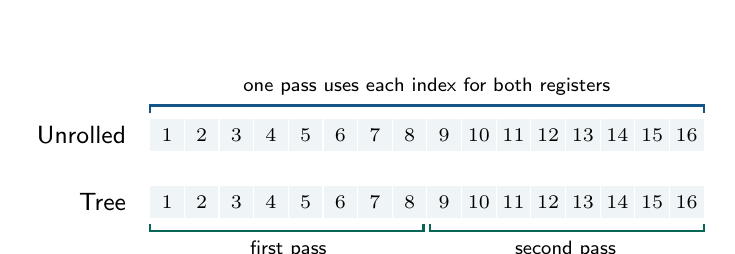
\begin{tikzpicture}[x=.44cm,y=.85cm]
\foreach \y/\name in {1/Unrolled,0/Tree}{
\node[anchor=east,font=\sffamily\small] at (-.4,\y) {\name};
\foreach \i in {0,...,15}{
\pgfmathtruncatemacro{\n}{\i+1}
\filldraw[draw=white,fill=panel] (\i,\y-.25) rectangle ++(1,.5);
\node[font=\scriptsize] at (\i+.5,\y) {\n};}}
\draw[thick,outA] (0,1.32)--(0,1.44)--(16,1.44)--(16,1.32);
\node[above,font=\sffamily\scriptsize] at (8,1.44) {one pass uses each index for both registers};
\draw[thick,outC] (0,-.33)--(0,-.44)--(7.9,-.44)--(7.9,-.33);
\draw[thick,outC] (8.1,-.33)--(8.1,-.44)--(16,-.44)--(16,-.33);
\node[below,font=\sffamily\scriptsize] at (4,-.44) {first pass};
\node[below,font=\sffamily\scriptsize] at (12,-.44) {second pass};
\end{tikzpicture}
\end{center}

The parameter \(M\) counts activation rows; \(L\) counts columns in a weight
block. For \(L=3\) with AVX2 available the paths are:
\[
\begin{array}{c|l|l}
M&\text{SSR unrolled}&\text{SSR tree}\\\hline
1&1\text{ scalar row}&1\text{ scalar row}\\
8&8\text{ scalar rows}&1\text{ batch of }8\\
16&1\text{ batch of }16&2\text{ batches of }8\\
18&1\text{ batch of }16+2\text{ scalar rows}&
2\text{ batches of }8+2\text{ scalar rows}
\end{array}
\]
A tail is the remainder after complete batches. For widths \(1,7,8\), tree
delegates to unrolled. Without an enabled and available AVX2 path, both
wrappers use scalar computation. Thus differently named curves can time the
same code. The benchmark records the backend, including mixed vector/scalar
tails. Optional OpenMP assigns rows or complete batches to different threads.
SIMD works inside a batch on one core. At \(M=16\) the unrolled vector loop
has only one batch for OpenMP to assign. The local wrappers also handle
rectangular strides and crop padded output columns before returning \(Y\).

\Needspace{7\baselineskip}
\section{Why benchmark these SSR variants?}
Basic already skips the zero group. Comparing basic with RSR++ illustrates
the effect of that choice together with their different folding loops and
working buffers. Comparing basic with unrolled keeps groups fixed and tests
batch SIMD and two-way unrolling together. Comparing unrolled with tree
then tests a generic vector reduction against fixed-width updates. This
last pair changes both reconstruction and batch size, so a timing difference
cannot uniquely identify which change was responsible.

The pinned upstream header also declares an FP32 eight-row variant
with the suffix \code{unroll8_v2}, FP32 specializations for
\(L=7,8\), and integer kernels \cite{ssrup}. The eight-row generic implementation uses a single vector batch per iteration;
comparison with the 16-row variant changes the number of batches handled together.
The current three entries already cover a scalar reference, a generic
16-row kernel and an eight-row specialized kernel. The wider specializations
answer a width-specific question: spelling out each pattern requires 127
or 255 cases per plane instead of 63 at \(L=6\). The default sweep uses
width six. Integer variants would change the activation type or require
quantizing the FP32 inputs, changing the numerical question as well.

At the default \(M=16,L=6\), both optimized paths can run on AVX2 hardware.
The same prepared weights, input data and FP64 validation keep the
mathematical task common. Report the width, batch size, backend and thread
setting alongside the timing. Preprocessing and stored bytes are reported
separately; API time includes internal allocations and output copies.
These properties motivate the comparison without assuming a speed ranking
for unmeasured alternatives.

\Needspace{14\baselineskip}
\familymark{Ternary Compressed Sparse Column}
\Needspace{7\baselineskip}
\section{TCSC: computing one output column from two lists}\label{sec:tcsc}
Ternary Compressed Sparse Column (TCSC) starts with a question about
one output: which inputs should we add, and which should we subtract?
The weights determine the answer before the first input arrives
\cite{tcscpaper}. Keep the column labels \(\abc{A}{B}{C}\). For one input row,
take
\[
\mathbf{x}=\begin{bmatrix}2&3&5&7&11\end{bmatrix},\qquad
W=\begin{weights}
 1& 0&-1\\
 0&-1& 1\\
-1& 0& 0\\
 1& 1& 0\\
 0& 0& 1
\end{weights}.
\]
Read the blue column downward. The first weight tells us to add \(x_1\),
the third to subtract \(x_3\), and the fourth to add \(x_4\). We can
therefore replace the entire column by two lists:
\[
P_A=[1,4],\qquad N_A=[3],\qquad
\ca{y_A}=(x_1+x_4)-x_3=(2+7)-5=4.
\]
In general, define \(P_j=\{k: W_{kj}=+1\}\) and \(N_j=\{k:W_{kj}=-1\}\).
Here the subscript in \(N_j\) denotes a negative-index list; \(N\) alone
is the total number of output columns. The same identity holds for every
row \(i\) of a batch:
\[
Y_{ij}=\sum_{k\in P_j}X_{ik}-\sum_{k\in N_j}X_{ik}.
\]
For our single input, all three columns fit on one line each:
\[
\begin{array}{c|l|l|l}
j&P_j&N_j&y_j\\ \hline
\ca A &[1,4]&[3]&\ca{x_1+x_4-x_3=4}\\
\cb B &[4]&[2]&\cb{x_4-x_2=4}\\
\ccol C &[2,5]&[1]&\ccol{x_2+x_5-x_1=12}
\end{array}
\]
When another input arrives, the lists stay the same. Only the values
read from that input change. For example, \(x_4\) contributes to both
\(A\) and \(B\), so its index occurs in both positive lists. RSR and SSR
can group input rows that share an entire weight pattern and reuse their
sum across columns. TCSC instead enumerates each column's nonzeros
directly. This makes it a useful comparison when sparsity is high but
the surviving patterns repeat infrequently.

\Needspace{5\baselineskip}
\subsection{From the lists to the four arrays in the paper}
Place the positive lists back to back in column order, then repeat for
the negatives. The bars below show boundaries; each stored index takes
part in exactly one list per occurrence.
\[
\begin{aligned}
\text{positive row indices}&=[\,\ca{1,4}\mid\cb 4\mid\ccol{2,5}\,],
&\text{positive offsets}&=[0,2,3,5],\\
\text{negative row indices}&=[\,\ca 3\mid\cb 2\mid\ccol 1\,],
&\text{negative offsets}&=[0,1,2,3].
\end{aligned}
\]
As in the earlier examples, the displayed row labels start at one. Offsets
are zero-based positions within an index array. For column \(C\), the
positive offsets give the interval \([3,5)\). Positions 3 and 4 contain
row labels 2 and 5. The negative interval \([2,3)\) contains row label
1. This recovers \(x_2+x_5-x_1\). Equal adjacent offsets denote an empty
list. The extra offset at the end closes the last column.

Ordinary CSC stores a value alongside each nonzero row index. In basic
TCSC the choice of list already supplies that value's sign. A zero supplies
no index. For our 15 weights the index arrays contain eight entries in
total, one per nonzero. With the local 32-bit indices and offsets, basic's
array payload alone is \(4[8+2(3+1)]=64\) bytes. In general it is
\(4[\mathrm{nnz}+2(N+1)]\) bytes when the offsets are 32-bit. On such a tiny
matrix pointers take a large fraction of the space. For large \(K\), the
number of nonzeros per column matters much more. Compression in bytes depends on both index width and sparsity. The local
kernels use 32-bit row indices \cite{tcsclocal}.

\Needspace{7\baselineskip}
\section{What the two TCSC kernels do on the CPU}
\Needspace{5\baselineskip}
\subsection{TCSC basic: consume a positive and a negative in one loop}
The scalar kernel reads both lists for one column. As long as both have
an entry, it subtracts one activation and adds one in the same iteration.
For \(\ca A\) the first iteration gives \(0-x_3+x_1=-3\). The positive
list has one entry left, so the remainder adds \(x_4=7\), giving 4.
The following shortened code uses zero-based row indices as in C++.
Here \code{pos} and \code{neg} point to the starts of this column's lists.
\Needspace{11\baselineskip}
\begin{lstlisting}
float sum = 0;
int pairs = std::min(npos, nneg);
for (int k = 0; k < pairs; ++k) {
    sum -= x[neg[k]];
    sum += x[pos[k]];
}
for (int k = pairs; k < npos; ++k) sum += x[pos[k]];
for (int k = pairs; k < nneg; ++k) sum -= x[neg[k]];
\end{lstlisting}
Pairing requires no shared row between the two indices. They simply update
the same output. For a column with 100 entries of each sign, the paired loop
makes 100 iterations for 200 contributions. It still needs 200 activation
reads and 200 arithmetic updates. The potential saving is loop control.
For a column of one sign only, the remainder loop does all the work.

\Needspace{5\baselineskip}
\subsection{TCSC merged: organize pairs across columns}
First rewrite the same three outputs as a paired part plus a remainder:
\[
\begin{aligned}
\ca{y_A}&=(x_1-x_3)+x_4,\\
\cb{y_B}&=(x_4-x_2),\\
\ccol{y_C}&=(x_2-x_1)+x_5.
\end{aligned}
\]
The first pair in every column has the same arithmetic shape. Line up
the first positive indices across columns and do the same for the negatives:
\[
 [\abc{x_1}{x_4}{x_2}]-[\abc{x_3}{x_2}{x_1}]
 =[\abc{2}{7}{3}]-[\abc{5}{3}{2}]=[\abc{-3}{4}{1}].
\]
Now add the residual contributions
\([\abc{x_4}{0}{x_5}]=[\abc{7}{0}{11}]\). The result is
\(\mathbf y=[\abc{4}{4}{12}]\), exactly as in the basic example.

The three columns illustrate the ordering on paper. The real SIMD path
requires a complete group of \emph{eight} columns. In the local
\code{1xG8} kernel each group handles one input row at a time; its
eight lanes hold columns \(A,\ldots,H\) of that row. In SSR unrolled
the eight lanes held eight input rows. This difference determines which
matrix dimension must be large enough to fill a vector.

\paragraph{How many rounds fit in one group?}
Let \(p_j=|P_j|\) and \(n_j=|N_j|\) for each column in the group \(G\).
Column \(j\) can supply \(\min(p_j,n_j)\) pairs. To fill every lane,
the GroupMin layout takes
\[
q_G=\min_{j\in G}\min(p_j,n_j).
\]
If the eight pair counts are \((5,4,6,5,4,7,5,6)\), then \(q_G=4\).
Four full vector rounds handle \(4\cdot8\cdot2=64\) nonzero contributions
per input row. Next the kernel finishes the positive and negative remainders
for each column. Those remainders may include \emph{both} signs: a column
with seven possible pairs has consumed only four. If one column has six
positives and zero negatives, its pair count is zero, and the entire group
uses the remainder path. A matrix's global zero fraction cannot reveal
how much work will run in the common vector loop.

\Needspace{5\baselineskip}
\subsection{Loading indices, gathering activations and accumulating}
Preprocessing lays out one common round as eight positive row indices
followed by eight negative row indices. This is the non-interleaved
GroupMin option used by the wrapper. It also records two offsets for the
common interval and two remainder endpoints for each column: 18 metadata
entries per group. The hot loop can now read two consecutive chunks of index
data. The activations selected by those indices may still be far apart.
\Needspace{9\baselineskip}
\begin{lstlisting}
// One common round, abbreviated from the AVX2 kernel
idx_p = load_8_int32(row_index + k);
idx_n = load_8_int32(row_index + k + 8);
pos = _mm256_i32gather_ps(x, idx_p, 4);
neg = _mm256_i32gather_ps(x, idx_n, 4);
acc = _mm256_add_ps(acc, _mm256_sub_ps(pos, neg));
\end{lstlisting}
For one lane, the address selected by the positive gather is
\[
\operatorname{address}(x[{\rm idx}_p[\ell]])
 = \operatorname{base}(x)+4\,{\rm idx}_p[\ell]\quad\text{bytes}.
\]
For example, in column \(A\) the printed row label 1 is stored as C++ index
0 and row label 3 as index 2. The positive gather reads the first float,
the negative gather reads the third, and their difference is \(-3\).
The remainder subsequently adds \(x_4=7\), producing the final \(4\).

The gathers translate two rows of packed indices into two vectors of activations. The
three-column teaching example uses the same ordering as an eight-lane group:
\begin{center}
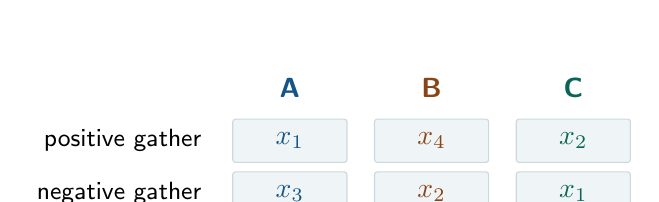
\begin{tikzpicture}[x=1cm,y=.67cm,
 cell/.style={draw=rulegray,rounded corners=1pt,fill=panel,minimum width=1.45cm,minimum height=.55cm}]
\foreach \xx/\name/\p/\n/\col in {0/A/1/3/outA,1.8/B/4/2/outB,3.6/C/2/1/outC}{
\node[font=\sffamily\bfseries,text=\col] at (\xx,1) {\name};
\node[cell,text=\col] at (\xx,0) {\(x_{\p}\)};
\node[cell,text=\col] at (\xx,-1) {\(x_{\n}\)};}
\node[anchor=east,font=\sffamily\small] at (-1,0) {positive gather};
\node[anchor=east,font=\sffamily\small] at (-1,-1) {negative gather};
\end{tikzpicture}
\end{center}
Read \emph{across} a row to see which activations a gather retrieves. Read
\emph{down} a column to see the difference accumulated in one lane.

The first two lines abbreviate unaligned vector loads. A gather takes eight
indices and retrieves the corresponding eight floats from the current input
row. The scale 4 converts a float index to a byte offset. Lane \(A\)
therefore receives \(x_1-x_3\) in the first round of our example. Other
lanes compute their own column's difference with the same instruction.
The register \code{acc} keeps eight partial results across rounds. After
one vector store to adjacent output columns, scalar loops finish the
remainders. Irregular reads can still miss the cache, so grouping improves
the organization of indices and arithmetic without guaranteeing faster
activation loads. FP32 rounding can differ from basic because the additions
are associated differently.

\paragraph{Threads, incomplete groups and fallback.}
Optional OpenMP assigns whole columns to threads in basic and complete
eight-column groups in the merged vector loop. Each thread owns distinct
outputs. At \(N=1024\) there are 128 groups available even when \(M=1\).
SIMD works within a group; threads can work on different groups.
At \(N=19\), two groups cover columns 1--16 and a scalar tail handles
17--19. This \emph{column tail} is separate from the \emph{index remainders}
within a complete group. At \(N<8\) only the scalar tail executes on the
AVX2 path. If AVX2 is unavailable or disabled, the wrapper calls basic.
The group size is fixed at eight independently of the RSR/SSR width setting.

\Needspace{7\baselineskip}
\section{Why benchmark these two TCSC kernels?}
Both compute the same FP32 row-major product on arbitrary ternary weights.
Basic measures the benefit of visiting only the nonzeros with implicit signs.
Merged tests whether eight-column packing, gathers, and SIMD arithmetic repay
their costs on the same matrix. The pair fits rectangular shapes and remains
usable at \(M=1\). Comparing them changes both layout and execution, so any
measured difference belongs to the combination. In the local benchmark both
entries share one preprocessing call and one weight object retaining basic
\emph{and} merged arrays. Their reported setup time and stored bytes therefore
describe that shared object; they cannot be used to estimate the standalone
format sizes from the paper.

The pinned upstream CPU sources offer several other experiments \cite{tcscup}.
The choices below explain the scope of the comparison and what an additional
kernel would measure.
\begin{itemize}
\item \textbf{Row-major basic and one-row GroupMin.} Both consume the same
activation layout as the rest of the benchmark. The upstream row-major
\(2{\times}G8\) and \(4{\times}G8\) routines also tile over input rows.
They would help measure metadata reuse across a larger batch; the selected
\(1{\times}G8\) exposes the effect of grouping columns with a single input.
The row-major scalar \(4{\times}4\) unroll would test loop tiling separately.
\item \textbf{Eight columns versus larger groups.} Eight FP32 values fit
one AVX2 register. Upstream also offers \(G16\) and \(G32\) variants.
Extending a group can only keep or reduce its minimum pair count. Larger
groups therefore trade a different tiling strategy against the possible loss
of common rounds. Their performance depends on the distribution of signs.
\item \textbf{GroupMin versus padded or uniform layouts.} GroupMin works
with unequal column lengths and stores only real contributions in its common
interval. The upstream GroupMid design can extend that interval with cancelling
pairs \(x_k-x_k\); regularity costs extra entries and reads. Uniform TCSC
targets matrices with the same counts of positive and negative entries
per column within a tile and fully paired columns. The benchmark's arbitrary ternary
weights do not guarantee that structure.
\item \textbf{Different layouts, instruction sets or precision.} Upstream
column-major implementations, AVX-512 variants and INT8 kernels answer
questions about different memory layouts, hardware capabilities or activation
types. Using row-major FP32 keeps the numerical task and data representation
consistent with the existing inputs. The selection establishes a portable
reference and an optimized x86 comparison; it implies no speed ranking of the
unmeasured variants.
\end{itemize}

\clearpage
\familymark{Benchmark interpretation}
\Needspace{7\baselineskip}
\section{Reading a CPU benchmark result}\label{sec:timing}
A benchmark row identifies a mathematical task, a kernel implementation and an
execution path. Compare the columns of the CSV in that order. As a running
example, consider the default sweep case \(M=16,K=N=1024,b=6\).
\Needspace{5\baselineskip}
\subsection{Where one instruction and one thread do work}
The table counts independent units in the main loop for this example.
For vector entries assume the indicated SIMD backend is active. OpenMP
must also have been enabled at compilation for that outer loop to use threads.
\begin{center}
\small
\begin{tabular}{@{}p{.22\linewidth}p{.34\linewidth}p{.36\linewidth}@{}}
\toprule
Entry & Meaning of one SIMD lane & Work available to OpenMP\\ \midrule
RSR, RSR++ & Portable scalar source & Sequential reference calls\\
RSR-core & v3.3 vector path: one output column in one input row &
\(\lceil1024/6\rceil=171\) blocks per input row and pass\\
SSR basic & Scalar source & 16 independent input rows\\
SSR unrolled & One input row for one output & \(16/16=1\) full batch\\
SSR tree & One input row for one output & \(16/8=2\) full batches\\
TCSC basic & Scalar source & 1024 output columns\\
TCSC merged & One output column in one input row &
\(1024/8=128\) full groups\\
\bottomrule
\end{tabular}
\end{center}
The length-1--4 switch and four scalar accumulators for one group occur
in all three RSR-core variants. The lookahead on paths with explicit
prefetch is 64 permutation entries in v4.2 and 48 in v3.1 and v3.3.
Portable RSR and RSR++, TCSC and SSR have no corresponding explicit
prefetch loop here. SSR unrolled keeps separate vector totals for batches
of input rows, while TCSC merged accumulates contributions for eight
output columns. The OpenMP column above describes how work is divided
between threads independently of those within-thread operations.

For example, with four requested threads the SSR unrolled main loop has a
single iteration. A thread can still issue vector instructions within that
iteration. TCSC merged can divide its 128 groups among four workers; their
actual running times also depend on how many nonzeros those groups contain.
The environment settings in the CSV record requested threads. They do not
measure core occupancy.

\Needspace{5\baselineskip}
\subsection{What a time or speedup means}
The harness validates against an FP64 reference, calibrates batches to warm
the kernels, shuffles the order across samples, and reports the median of
per-call batch averages. Its recorded speedup is
\[
 S_{\rm BLAS} = T_{\rm BLAS}/T_{\rm kernel}.
\]
Thread scaling asks a separate question. For the same kernel, problem,
backend and binary, \(S_t=T_1/T_t\) compares one requested thread with \(t\).
For example, a hypothetical drop from \(80\) to \(50\,\mu\mathrm{s}\) gives
\(S_t=1.6\). Both numbers must come from the same scope of work.
The validation tolerance accounts for FP32 rounding, including reassociation
of sums. The measured call includes internal allocation and required output
copies. Preprocessing and retained weight bytes appear separately. If weights
are used for \(R\) products, the average cost including preparation is
approximately \(T_{\rm call}+T_{\rm prep}/R\). This distinction explains
why inference timing and one-off multiplication can favor different formats.

The dense BLAS entry delegates to OpenBLAS; Eigen CSR and CSC delegate their
products to Eigen. Their internal dispatch is library-specific. A scalar
label for a custom kernel describes its arithmetic path, and can coexist
with OpenMP parallelism. The code and build settings for these distinctions
are in \code{Makefile}, \code{src/benchmark.cpp} and the registration in
\code{include/baseline_suite.h} \cite{local}.

\clearpage
\begin{thebibliography}{99}
\bibitem{paper} M. Dehghankar, M. Erfanian and A. Asudeh.
\emph{An Efficient Matrix Multiplication Algorithm for Accelerating Inference
in Binary and Ternary Neural Networks}, Sections 3 and 4.
\href{https://arxiv.org/html/2411.06360v3}{arXiv:2411.06360v3}.
\bibitem{core} UIC-InDeXLab.
\href{https://github.com/UIC-InDeXLab/RSR-core/tree/99bcccded70416839f1ef1fc6d58726c507d1fb9/kernels}{RSR-core kernel sources at the revision imported by this project}
(commit \code{99bcccd}, MIT).
\bibitem{guide} UIC-InDeXLab.
\href{https://github.com/UIC-InDeXLab/RSR-core/blob/main/docs/OPTIMIZATION.md}{RSR Multiplier Optimization Guide}, binary and ternary CPU sections.
\bibitem{ssrpaper} A. Pittet, S. Zhu, V. Verdan and G. Alonso.
\href{https://arxiv.org/html/2610.08403v1}{SSR: Sparse Segment Reduction for Ternary GEMM Acceleration}, DATE 2026, Section III.
\bibitem{ssrup} ETH Zurich, FPGA @ Systems Group.
\href{https://github.com/fpgasystems/ternaryLLM/blob/68d384425261d60bfbde5ff079c33a474c1eb28e/SSR/SSR/ssr_vec.h}{FP32 and integer kernel declarations},
\href{https://github.com/fpgasystems/ternaryLLM/tree/68d384425261d60bfbde5ff079c33a474c1eb28e/SSR/SSR}{SSR sources at the imported revision}.
\bibitem{ssrlocal} Project SSR source map: \code{src/baselines/ssr_baseline.cpp},
functions \code{handle_block_ssr}, \code{ssr_inference_rows},
\code{ssr_inference_float_vec_unroll16_v2}, the width-specific L2--L6
functions, and \code{multiply_tree}. Registration is in \code{include/baseline_suite.h}.
\bibitem{local} Project source map:
\code{src/baselines/rsr.cpp} (portable inference, \code{step_three}, imported
kernels and weight preparation);
\code{include/baseline_suite.h} (registration, plane splitting and workspace);
\code{src/benchmark.cpp} and \code{README.md} (timing scope and validation).
\bibitem{tcscpaper} S. Zhu, G. Fu, M. Kjoseva and G. Alonso.
\href{https://doi.org/10.1145/3807782}{Efficient Addition-Based Sparse GEMM for Fast Ternary Large Language Model Inference on Edge Devices}, ACM TECS, 2026.
\bibitem{tcscup} ETH Zurich, FPGA @ Systems Group.
\href{https://github.com/fpgasystems/ternaryLLM/blob/68d384425261d60bfbde5ff079c33a474c1eb28e/ternaryLLM_CPU/src/GEMM_CPU_FP32.hpp}{Upstream FP32 CPU kernel inventory}
and \href{https://github.com/fpgasystems/ternaryLLM/blob/68d384425261d60bfbde5ff079c33a474c1eb28e/ternaryLLM_CPU/src/TCSC.hpp}{TCSC layouts at the imported revision}.
\bibitem{tcsclocal} Project TCSC source map:
\code{src/baselines/tcsc_baseline.cpp} (packing, scalar paired loop,
GroupMin gathers, column tail and dispatch);
\code{include/baseline_suite.h} (shared preparation and backend labels).
\end{thebibliography}
\end{document}
